%=================
\chapter{Sprint 4}
%=================
This chapter contains the description of the work done in sprint 4. The 
chapter is diveded into sprint planning in \autoref{sec:sp4:planning}, design 
done during the sprint in \autoref{sec:sp4:design}, the implementation in 
\autoref{sec:sp4impl}, the result of the sprint testing in 
\autoref{sec:sp4test}, feedback the customer gave us during the sprint in 
\autoref{sec:sp4feedback} and evaluation of the sprint in 
\autoref{sec:sp4eval}.

%------------------------
\section{Sprint Planning}
%------------------------
\label{sec:sp4:planning}
The fourth sprint will be the last iteration of this project. Because it is very important to make the \gls{utility} work properly on Thales' source code, most of the sprint work hours will be used on testing and bugfixing. Now the \gls{utility} fails on most of the \glspl{struct}; the customer tried to generate \glspl{dissector} for 580 \glspl{struct}, and only 4 of them succeeded. It will probably take som time to fix the issues in the customer code.

We know that some of our earlier implementation do not work as intended or are incomplete. The customer has given us feedback on the fulfilled requirements, and pointed out what needs to be improved. These are important work items that were added to this sprint backlog \ref{tab:sprint4req}. In addition, we received new requirements that the customer would like us to implement, as they add some convenient functionalities for them. For the optional requirements that we might not have time to implement, we have agreed to write a specification on how to implement them. 

There will not be another sprint after this one, so we can not postpone any work items. Because of this, we had to make some of the new requirements from the customer optional, and also told he customer that we will probably not be able complete all their desires. We are trying to improve from the last sprint, and will therefore not add more tasks than we think we can complete this sprint. This sprint we plan to use close to 350 hours, but it is still likely that we will use more and are prepared for that. There will certainly pop up new tasks and unforeseen bugs that we have to fix.

\subsection{Duration}
%-----------------------
The sprint started with the planning meeting the 2nd of November and our work started the following day. The sprint duration is 14 days, and will end on the 15th of November with a review meeting. 

\subsection{Sprint Goal}
%-----------------------
The goal of this sprint will be to focus on fixing and implementing functions that the customer will need to use the \gls{utility} on their source code. The most important thing to focus on in the beginning of the sprint will be to implement support for \#pragma directives and support for including \gls{header}-files that are not included by the \gls{preprocessor}. This is important, as it will make it possible for the customer to fully test the \gls{utility}.

Since the deadline of the project is 24th November, there will also be a focus on preparing a presentation and improving the report for the final delivery. The team are also going to hold a presentation for the customer's developers on the 17th of November, and it is important to also focus on this presentation.

\subsection{Back Log}
%--------------------
This section contains the sprint backlog in \autoref{tab:sprint4req} and the timetable for the sprint in \autoref{tab:sprint4time}.  

\begin{table}[!htbp] \small \center
\caption{Sprint 4 Requirement Work Items \label{tab:sprint4req}}
\begin{tabularx}{\textwidth}{l X c c}
	\toprule
	User & & \multicolumn{2}{c}{Hours} \\
	\cmidrule(r){3-4}
	story & Req. and Description & Est. & Act. \\
	\midrule
	\textbf{Impl.} &  & \textbf{47} & \textbf{24} \\
	\hyperref[tab:req:stories13]{US56} & FR2-E: Guess \gls{dissector} from \gls{packet} size & 5 & 3 \\
 	\hyperref[tab:req:stories10]{US40} & FR3-A mod: Support \gls{include} of system \glspl{header} &  8  & 3 \\
	\hyperref[tab:req:stories10]{US41} & FR3-D mod: Ignore \#pragma directives & 2 & 1 \\
	\hyperref[tab:req:stories10]{US42} & FR3-E: Find include dependencies which are not explicitly set & 16  & 11 \\
	\hyperref[tab:req:stories11]{US47} & FR4-B mod: Custom \Gls{lua} files support inside a .cnf file & 4 & 1 \\
	\hyperref[tab:req:stories12]{US49} & FR4-D mod: Multiple message ID's for one \gls{dissector} & 2 & 1 \\
	\hyperref[tab:req:stories12]{US52} & FR4-H: Autogenerate configuration files for \glspl{struct} without a config file & 1  & 0.5\\
	\hyperref[tab:req:stories12]{US51} & FR4-I: Allow configuration of size for unknown \glspl{struct} & 4 & 1 \\
	\hyperref[tab:req:stories10]{US43} & FR6-E: Support \Gls{c} macros from \gls{cli} & 1 & 1 \\
	\hyperref[tab:req:stories12]{US54} & FR6-F: Only generate \glspl{dissector} for \glspl{struct} with valid a id and their dependencies & 4 & 1.5 \\
	\addlinespace
	\textbf{Fixes} &  & \textbf{35} & \textbf{43.5} \\
	& TheFIX: Be able to process customer's files & 12 & 17 \\
	 & FR2-A: Improve generated \Gls{lua} output & 10 & 20 \\
	 & FR1-E: \Gls{array} bug in text & 2 & 1.5 \\
	 & FR1-E: Pointer support (array) & 1 & 0.5 \\
	 & FR1-E: \Gls{enum} in \glspl{array} & 1 & 1 \\		
	 & FR6-C: \Gls{batch mode} (recursive search for subfolders) &  8  & 2 \\
	 & FR6-C: Support command line arguments for Cpp & 1 & 0.5\\
	 & Exclude certain folders and files in batch mode & 1 & 1 \\
	\addlinespace
	\textbf{Testing} &  & \textbf{16} & \textbf{7.5} \\
	 & Fixing existing tests & 3 & 3.5 \\
	 & Add more tests for csjark module & 3 & 1 \\
	 & Add more tests for cparser module & 3 & 0.5 \\
	 & Add more tests for the config module & 2 & 0.5 \\
	 & Add more tests for the dissector module & 2 & 0.5 \\
	 & Add more tests for platform module & 1 & 0 \\
	 & Add sprint 4 end-to-end tasks & 2 & 1.5 \\
	\addlinespace
	\textbf{Doc.} &  & \textbf{15} & \textbf{17.5} \\
	\hyperref[tab:req:stories10]{US44} & Update command line interface document & 1 & 1 \\
	\hyperref[tab:req:stories11]{US48} & Update user documentation for custom \Gls{lua} & 1 & 1.5 \\
	\hyperref[tab:req:stories12]{US50} & Update user documentation for message ID & 1 & 1 \\
	\hyperref[tab:req:stories12]{US53} & User documentation for \gls{struct} size configuration & 1 & 1 \\
	\hyperref[tab:req:stories12]{US55} & User documentation for generating only \gls{struct} with valid ID or dependencies & 1 & 1 \\
	\hyperref[tab:req:stories9]{US36} & Which platforms that the \gls{utility} supports & 2 & 1 \\
	\hyperref[tab:req:stories13]{US58} & How to define new platforms to support & 1 & 3.5 \\
	\hyperref[tab:req:stories9]{US37} & Create developer manual from python docstrings & 2 & 2 \\
	& Updates and polishing & 5 & 5.5 \\
	\midrule
	& Total: & 113 & 92.5 \\
	\bottomrule
\end{tabularx}
\end{table}

\begin{table}[!htb] \small \center
\caption{Sprint 4 Timetable\label{tab:sprint4time}}
\begin{tabularx}{\textwidth}{X c c}
	\toprule
	& \multicolumn{2}{c}{Hours} \\
	\cmidrule(r){2-3}
	Description & Est. & Act. \\
	\midrule
	\textbf{Sprint planning} & \textbf{30} & \textbf{27} \\
	\addlinespace
	\textbf{Sprint 4 requirements} & \textbf{113} & \textbf{92.5} \\
	Implementation & 47 & 24 \\
	Fixes & 35 & 43.5 \\
	Testing & 16 & 7.5 \\
	User Documentation & 15 & 17.5 \\
	\addlinespace
	\textbf{Sprint review} & \textbf{20} & \textbf{20} \\
	\addlinespace
	\textbf{Sprint documentation} & \textbf{46} & \textbf{52.5} \\
	Sprint 3 document & 4 & 4 \\
	Sprint 4 document & 42 & 48.5 \\
	\addlinespace
	\textbf{Report work} & \textbf{38} & \textbf{49} \\
	Update tables with actual hours & 2 & 2 \\
	Abstract - improve & 2 & 3\\
	Importing user documentation to report & 3 & 11 \\
	Introduction section & 6 & 10 \\
	Report read-through from a technical perspective & 6 & 6\\
	Report read-through from a non-technical perspective & 6 & 7\\
	Glossary refinement & 3 & 3\\
	Acronym refinement & 1 & 1\\
	Write about optional requirements & 4 & 2\\
	References & 3 & 2\\
	Requirement agreement & 2 & 2\\
	\addlinespace
	\textbf{Thales presentation} & \textbf{28} & \textbf{28} \\
	\addlinespace
	\textbf{Meetings} & \textbf{63} & \textbf{48.5} \\
	Advisor meetings & 28 & 20 \\
	Customer meetings & 14 & 10 \\
	Stand-up meetings & 21 & 18.5 \\
	\addlinespace
	\textbf{Project management} & \textbf{17} & \textbf{27} \\
	\midrule
	Total: & 351 & 344.5 \\
	\bottomrule
\end{tabularx}
\end{table}

%----------------------
\section{System Design}
%----------------------
\label{sec:sp4:design}
The utility lacked the last, but also most essential implementation at the start of fourth sprint; ability to run customer's source code flawlessly. To achieve this, we had to add functionality to support custom cases and the possibility for automatic configuration.

The sprint design this sprint will not be as comprehensive as the design in the prior sprints. This is because of two reasons:
\begin{itemize}
	\item This was the last sprint, if we were to implement many new features we also had to use time for testing and writing documentation for them, which we did not have.
	\item The existing features had to be extensively tested and documented before the project was over, leaving little time for other work. Testing and bug fixing was essential this sprint.
\end{itemize}
After three sprints, the design was to a large degree set. Re-factoring introduced some new modules, but it was just to make the code more logic and to distribute it so testing can be done more easily. This is described in the system overview section.

\subsection{System overview}
%-----------------------
The addition of new requirements from the customer resulted in changes in the utility's system overview. The need for more custom handling ended in a re-factoring of the code. This is visible in the \autoref{fig:sp2class}, which was extended from the third sprint. Two new modules was added, cpp and fields. Major changes to the class diagram are described below. How the modules interact is described in \autoref{sec:sp4:design:md}.

\begin{figure}[ht]
	\center
	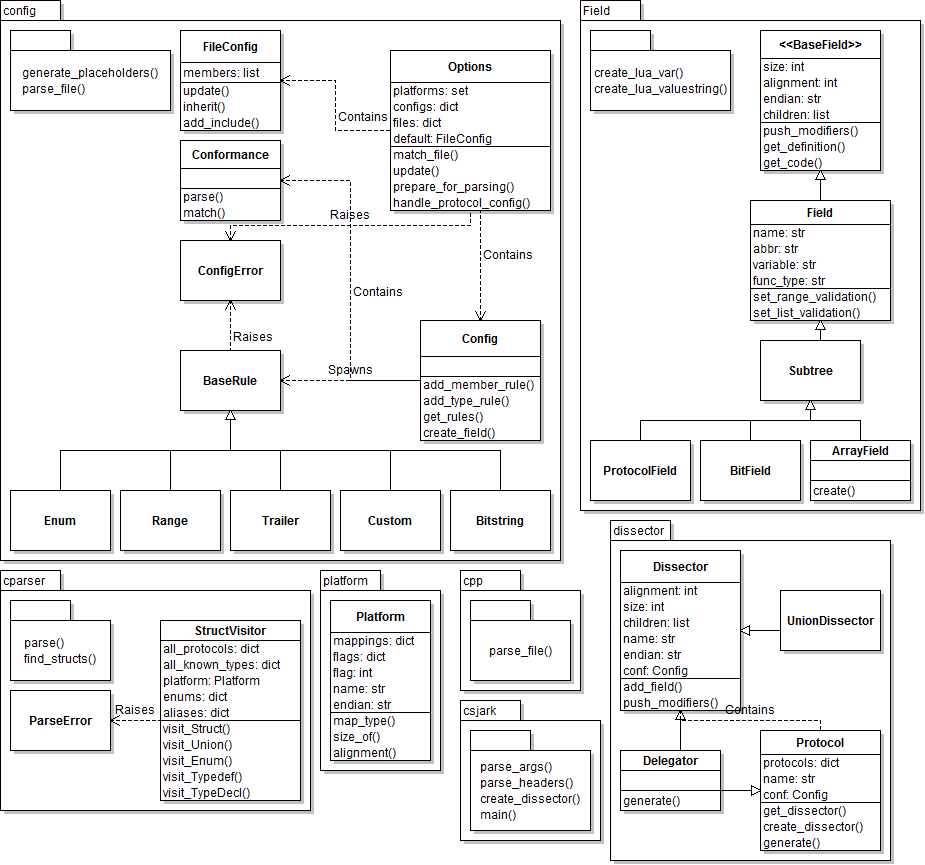
\includegraphics[width=\textwidth]{./sprints/img/ClassDiagramSprint4v2.png}
	\caption{Sprint 2 Class Diagram \label{fig:sp2class}}
\end{figure}

\subsubsection{ccp module}
The need for preprocessing C files before they are parsed have become so comprehensive, that we decided to create a dedicated module for it. All the existing cpp concerned code was relocated from the cparser module, and joint with the new implementation. The requirements listed in\autoref{tab:sprint4req}, made it necessary to have more functionality regarding the preprocessor step. 

\subsubsection{fields module}
Field specific classes were moved from the dissector module to its own, field. For the same reason as the ccp module; the amount of code concerning fields became so great, that a own module was appropriate. There was some refactoring in the field module. BaseField was added and has Field as a subclass. The class Field in is the most important class in this module, and generate the most of fields for the dissector. Subtree is a class that generates fields for the dissector, that will need a subtree in Wireshark, this class has three subclasses, BitField, ArrayField and ProtocolField.

\subsubsection{cparser module}
Some changes was done in this module due to the refactoring, functionality for the c preprocessing was moved. And some new methods was added since, field and dissector module was splitted. 

\subsubsection{config module}
The class FileConfig was added, to hold the configuration for specific header-files. Some methods was also added for automatic generation of header-files.

\subsubsection{dissector module}
There was several changes, all the Field classes was added to it's own module, to hold the information about the generation, the class Dissector was added to the module. UnionProtocol was renamed to UnionDissector.

\subsection{Module Diagram}
\autoref{fig:sp2module} shows the dependencies between the modules. The main 
module for the utility is csjark, which have the the main-method. This module 
uses config to parse and hold all the configuration, starts preprocessing in 
cpp module, and at the end uses cparser to parse the header-files. At the end 
it get all the ProtocolsFields from the field module, so the Lua dissectors 
can be written to file.

The cpp module uses the config module to read options given for the c 
preprocessing.

The config module uses the two modules field and dissector to create 
configured dissector fields. The platform moduled is read, to get de 
predefined platform configuration.

When cparser have parsed all the header files, it startes the generation of 
all the Lua dissectors. To do this generation the StructVisitor class depends 
on four modules, config, platform, dissector and field.

The dissector module uses the field module to generate fields for all the 
struct members. It also uses the platform module to get the correct sizes for 
the c types.

To get alignment sizes, the field module depend on the platform module.

\begin{figure}[ht]
	\center
	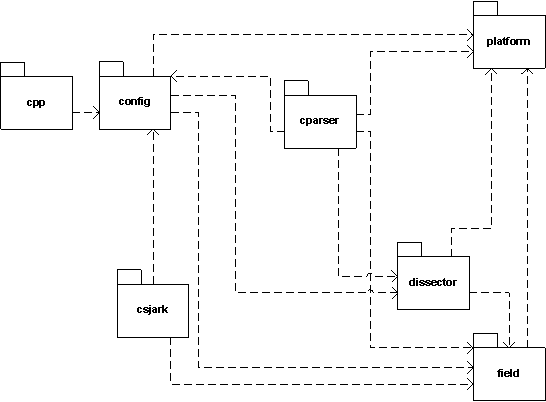
\includegraphics[width=\textwidth]{./sprints/img/sp4modulediagram.png}
	\caption{Sprint 2 Module Diagram \label{fig:sp2module}}
\end{figure}

\label{sec:sp4:design:md}

\subsection{User stories}
\label{sec:req:stories4}
This section lists the user stories for the fourth sprint, these are displayed in \autoref{tab:req:stories11}, \autoref{tab:req:stories12}, \autoref{tab:req:stories13} and \autoref{tab:req:stories14}.
As we are developing a very technical \gls{utility}, we have written user stories with an implementation level of abstraction. 
These user stories represent how we intend to add the functionality of each requirement to the \gls{utility}.
The administrator in this context is the administrator at Thales Norway AS. 
The developer is the person that uses \Gls{wireshark} with the \gls{dissector} generated by CSjark.

\begin{table}[htbp] \footnotesize \center
\caption{User stories - Sprint 4 part 1\label{tab:req:stories11}}
\noindent\makebox[\textwidth]{%
\begin{tabularx}{1.2\textwidth}{l X}
	\toprule
	Header & Value \\
	\midrule
	ID & US40 \\
	Requirement & FR3-A modification: \gls{include} system includes \\
	What & The \gls{utility} needs to be support system dependent \glspl{header}-files
	even if these are not available on the platform that the \gls{utility} is used on. \\
	How & The administrator is able to specify a fake system \gls{header} file with the defines they need to make their \glspl{struct} work correctly.
	This fake \gls{header} is then used to represent the system \gls{header} in the file so it is parsed correctly by \gls{pycparser}.  \\
	Result & The administrator is now able to make the \gls{utility} generate system dependent \glspl{dissector} for \glspl{header} with system dependent includes. \\
	\midrule
	ID & US41 \\
	Requirement & FR3-D: Ignoring \#pragma directives  \\
	What &  The \gls{utility} needs to be able to support \gls{header} files with the \#pragma directive without necessarily having to support the functionality of the directive\\
	How & Before feeding the \gls{header} files to the \gls{parser} the \gls{utility} needs to be able to run a pass through all of the \glspl{header} that are to be parsed and remove all of the \#pragma directives encountered in those \gls{header} files.\\
	Result & The user will be able to create \glspl{dissector} for \gls{header} files with the \#pragma directive instead of having the \gls{utility} be forced to skip them. \\
	\midrule
	ID & US42 \\
	Requirement & FR3-E: Find missing includes  \\
	What & It should be possible to generate \gls{dissector} from \gls{header}-files, that have definitions in \gls{header}-files that are not included with a \gls{preprocessor} directive in the \gls{header}-file.  \\
	How & The cparser module has to be able to detect when an exception is raised in the \gls{pycparser} \gls{library}, if an exception is raised, cparser has to search through the \gls{header}-files
	to find the declaration that the \gls{pycparser} \gls{library} failed on, and include this \gls{header} file. The cparser module will have to do this procedure until the \gls{dissector} is correctly parsed in the \gls{pycparser} \gls{library}. \\
	Result & The \gls{utility} shall be able to generate \glspl{dissector} for these \gls{header}-files \\	
	\midrule
	ID & US43 \\
	Requirement & Support \Gls{c} \glspl{define} from \gls{cli}  \\
	What & The administrator wants to pass \Gls{c} \gls{define} directives from the command-line to the \gls{preprocessor}.   \\
	How & When CSjark is executed, it takes the arguments given in the command-line interface and store them in the config module.
	The \gls{define} directives must be added to the \gls{preprocessor} arguments before the \gls{header}-file is parsed in the \gls{pycparser} \gls{library}.   \\
	Result & The \gls{utility} supports \Gls{c} \gls{define} directives passed from the \gls{cli}. \\
	\midrule
	ID & US44 \\
	User doc & Support \Gls{c} \glspl{define} from \gls{cli} \\
	What & The user wants to understand how the \gls{utility} will handle \Gls{c} \glspl{define} and what \glspl{define} that are possible to pass to the \gls{cli}.   \\
	How & The user finds the correct section in the user documentation, describing the command-line interface and how \Gls{c} \glspl{define} are handled.  \\
	Result & The user understands how to use \Gls{c} \glspl{define} with the \gls{utility}. \\
	\bottomrule
\end{tabularx}}
\end{table}

\begin{table}[htbp] \footnotesize \center
\caption{User stories - Sprint 4 part 2\label{tab:req:stories12}}
\noindent\makebox[\textwidth]{%
\begin{tabularx}{1.2\textwidth}{l X}
	\toprule
	Header & Value \\
	\midrule
	ID & US45 \\
	Requirement & FR7-A: Use Doxygen comments for ''Description''  \\
	What & The \gls{utility} will read Doxygen comments for a \gls{struct} and use that to specify the description field for the proto object in the \gls{dissector}. \\
	How & The \gls{utility} will search the \gls{header} files for Doxygen comments before giving the file to the \gls{preprocessor}. It will note what \gls{struct} the comment
	corresponds to and add it to the config module. The \gls{dissector} module will look up in the config module for each \gls{struct} and use the description field there if it has been found.  \\
	Result & The \glspl{dissector} now requires less manual configuration because it is able to use some of the text from the \gls{header} files. \\
	\midrule
	ID & US46 \\
	Requirement & FR7-B: Read \gls{int}-\gls{enum} config from \gls{header} files \\
	What &  The \gls{utility} will read \gls{define} statements that define the allowed values and the names corresponding to those values for integers that are to be treated like enums, so that the user will not have to configure them manually.\\
	How & The \gls{utility} will search the \gls{header} files for define statements that correpsonds to a \gls{member} that is configured to be handled as an \gls{enum}. The statements needs to follow some configurable format.
	These statements are then used to auto generate a configuration file for the \gls{int} \gls{member} used to make an \gls{enum} field for the \gls{int} \gls{member} when parsing the \gls{header} file.\\
	Result & The \gls{utility} now requires less manual configurations to make \glspl{dissector} interpret certain \glspl{integer} as \glspl{enum}. \\
	\midrule
	ID & US47 \\
	Requirement & Fetch offset in custom \Gls{lua} configuration  \\
	What & The administrator should be able to add configuration in the conformance file, so it is possible to add custom \Gls{lua} code with correct offset values.  \\
	How & The conformance file must support a variable for offset, and a way to use this. The config module have to read this variable, so it can be used in the \gls{dissector} module to generate a field in the \gls{dissector} that uses the correct offset. \\
	Result & The \Gls{lua} \gls{dissector} is generated with correct offset for the custom \Gls{lua} code. \\	
	\midrule
	ID & US48 \\
	User doc & Fetch offset in custom \Gls{lua} configuration  \\
	What & The administrator shall learn how to use offset values in custom \Gls{lua} configuration.   \\
	How & The administrator reads the section in the user documentation, about how to use custom \Gls{lua} in the \gls{utility}.  \\
	Result & The user will understand how to add offset values in the conformance file. \\
	\midrule
	ID & US49 \\
	Requirement & FR4-D modification: Support multiple message ID's for one \gls{struct} \\
	What & The administrator should be able to configure more than one message ID per \gls{struct}. Therefore it is possible to use the \gls{dissector} with several different messages (specified by different ID’s).    \\
	How & The configuration file must support definition of multiple ID’s. These ID’s then have to be used for registering multiple \glspl{protocol} for one \gls{dissector}.  \\
	Result & The \Gls{lua} \gls{dissector} can be used with multiple messages with different ID’s. \\
	\bottomrule
\end{tabularx}}
\end{table}

\begin{table}[htbp] \footnotesize \center
\caption{User stories - Sprint 4 part 3\label{tab:req:stories13}}
\noindent\makebox[\textwidth]{%
\begin{tabularx}{1.2\textwidth}{l X}
	\toprule
	Header & Value \\
	\midrule
	ID & US50 \\
	User doc & FR4-D modification: Support multiple message ID's for one \gls{struct}  \\
	What & The administrator should be able to find out how to specify multiple message ID’s for a specific \gls{struct}.
	This include the proper position and syntax of the message ID’s specification. Also, he should be aware of the consequences of that definition. \\
	How & The administrator reads the configuration section in the user documentation, about how to specify multiple message ID’s for a specific \gls{struct}.  \\
	Result & The administrator is able to specify and use multiple message ID’s for a specific \gls{struct}. \\
	\midrule
	ID & US51 \\
	Requirement & FR4-I: Allow configuration to specify the size of unknown \gls{struct} \glspl{member} \\
	What & The administrator should be able specify in the configuration, how big (in bytes) the \gls{struct} \gls{member} is without having the \gls{member} itself defined. Note: This is also a workaround for \glspl{struct} that are not parseable.\\
	How & The configuration should contain an optional attribute for each \gls{struct} \gls{member} which specifies the size of the \gls{member}. If this \gls{member} is a nested \gls{struct}, and this \gls{struct} is not defined, the size has to be specified. Otherwise the user should be informed about that.\\
	Result & The \Gls{lua} \gls{dissector} can be used with \Gls{c} \gls{header} that includes unspecified \gls{struct} \gls{member}. This \gls{member} was only defined by its size, so it could be displayed as raw data in \Gls{wireshark}. \\
	\midrule
	ID & US52 \\
	User doc & FR4-I: Allow configuration to specify the size of unknown \gls{struct} \glspl{member}  \\
	What & The administrator should be able to find out how to specify in the configuration, how big (in bytes) the \gls{struct} \gls{member} is without having the \gls{member} itself defined.  \\
	How & The administrator reads the configuration section in the user documentation, about how to specify the size of the \gls{struct} \glspl{member}. \\
	Result & The user is able to specify the size of unknown \gls{struct} \gls{member}. \\	
	\midrule
	ID & US53 \\
	User doc & Auto generate configuration files for \glspl{struct} with no corresponding configuration file \\
	What & The \gls{utility} will generate template configuration files if it encounters \glspl{struct} with no corresponding configuration file. This is to make it easier to make such a configuration file.   \\
	How & The cparser module checks if an encountered \gls{struct} has a corresponding configuration in the config module. If not, the \gls{utility} writes a template file for this \gls{struct}.   \\
	Result & The user will now be able to use the auto generated template file to write the configuration for a \gls{struct} instead of having to start from scratch. \\
	\midrule
	ID & US54 \\
	Requirement & Only generate \glspl{dissector} for \glspl{struct} that have a valid ID and their dependencies \\
	What & The \gls{utility} should only generate \glspl{dissector} for \glspl{struct} that have a configuration file with a valid ID and their dependencies.    \\
	How & When the \gls{utility} discovers a \gls{struct} definition inside a \gls{header} file it should check if there exists a configuration file for that \gls{struct} and if it has a valid ID.
	If not then the \gls{utility} should skip that \gls{struct} and continue with the \gls{header} file. If a \gls{struct} with a valid configuration file and ID has a \gls{member} that is not defined in the current \gls{header}
	file, then the \gls{utility} will check the includes in the current \gls{header} for the missing \glspl{struct} and create a \gls{dissector} for them as well.\\
	Result & The \gls{utility} will not generate \glspl{dissector} for \glspl{struct} which have not been specified in the configuration.
	This gives the users of the system the ability to specify which \glspl{struct} they want to look at as well as shortening the time the \gls{utility} needs to run. \\
	\bottomrule
\end{tabularx}}
\end{table}

\begin{table}[htbp] \footnotesize \center
\caption{User stories - Sprint 4 part 4\label{tab:req:stories14}}
\noindent\makebox[\textwidth]{%
\begin{tabularx}{1.2\textwidth}{l X}
	\toprule
	Header & Value \\
	\midrule
	ID & US55 \\
	User doc & Only generate \glspl{dissector} for \glspl{struct} that have a valid ID and their dependencies  \\
	What & The administrator should be able to specify in the configuration which \glspl{struct} should have \glspl{dissector} created for them. \\
	How & The administrator reads the configuration section in the \gls{utility}’s user documentation that specifies how to specify which \glspl{struct} should have a \gls{dissector} generated for them.  \\
	Result & The user will be able to specify which \glspl{struct} the \gls{utility} will generate \glspl{dissector} for. \\
	\midrule
	ID & US56 \\
	Requirement & Guess \gls{dissector} by \gls{packet} size \\
	What & The \gls{utility} should be able to generate a \Gls{lua} file that runs with \Gls{wireshark} and guesses the \gls{dissector} that is to be used for a \gls{packet}, if it has a message ID that does not match any pre-existing \gls{dissector}.\\
	How & The luastructs.lua file that is generated by the \gls{utility} should contain a dictionary of all \glspl{dissector}, sorted by the size of the \glspl{struct} that they are associated with.
 	When a \gls{packet} with an unrecognized message ID is discovered by \Gls{wireshark}, the code in the luastructs.\Gls{lua} file should try to match the unidentified \gls{packet} with a \gls{dissector}
 	that has been generated with the same size as the unidentified \gls{packet}. The matching \glspl{dissector} should then be run with the unidentified \gls{packet}. \\
	Result & Instead of only displaying the raw hex data from the unidientified \gls{packet}, \Gls{wireshark} should display the \gls{packet} as containing all of the possible \glspl{struct} and \gls{member} values the \gls{packet} might really be containing, as dictated by the matching \glspl{dissector}. 
	This \gls{packet} should also be displayed with a warning. \\
	\midrule
	ID & US57 \\
	Requirement & Display if \gls{struct} \gls{member} contains uninitialized memory \\
	What & The \glspl{dissector} generated by the \gls{utility} should be able to identify \gls{struct} \glspl{member} that might possibly have uninitialized memory set as their values.
 	These \glspl{member} and their values should be displayed with a warning in \Gls{wireshark} to indicate that the values might have been uninitialized.  \\
	How & If the \Gls{c}-code that uses \gls{header} files isn’t using memset to set the initial values of different variables a \gls{parser} might decide to fill uninitialized variables with some kind of patterned garbage data.
 	This pattern might be possible to detect by the \glspl{dissector} generated by the \gls{utility} by adding a check to the \gls{dissector} code which compares the \gls{member} values with different known garbage-patterns generated by different \glspl{parser}. \\
	Result & The \gls{utility} will now be able to generate \glspl{dissector} which will make \Gls{wireshark} display \gls{struct} \glspl{member} and their values with a warning if they are suspected as being filled with uninitialized memory. \\	
	\midrule
	ID & US58 \\
	User doc & How to define new platforms \\
	What & The Administrator should be able to define new platforms to support.  \\
	How & The user should look in the user documentation, and read the section about defining new platforms. \\
	Result & After the administrator has defined the new platform, the \gls{utility} should be able to generate \glspl{dissector} for the new platform. \\	
	\bottomrule
\end{tabularx}}
\end{table}

%-----------------------
\section{Implementation}
%-----------------------
\label{sec:sp4impl}
The implementation in this sprint has mainly been bug fixing, and adding 
features that the customer needs to be able to run the \gls{utility} on their code. 
This section covers the added functionality and the most important fixes 
in this sprint.

\subsection{Include Unsupported System-\glspl{header}}
%--------------------
CSjark must be able to support both Windows and Solaris operating system. To 
be able to generate dissectors from header-files, it was necessary to add 
system specific header-files for Windows and Solaris. This is done by adding 
the system-headers to the ''fake\_libc\_include''. ''fake\_libc\_include'' is 
a fake library for standard header-files, that only contains default typedefs 
and default defines. Most of the header-files in the fake library are empty, 
so the preprocessor can find the files that are included.

\subsection{Ignore \#pragma Directives}
%--------------------
Pragma directive is a \gls{preprocessor} directive that is used to give options to 
the compiler. This can for example be used to ignore warnings or give the 
compiler version-information of the code. Since the pycparser \gls{library} do not 
support pragma directives, these lines in the \Gls{c}-code is removed before the 
preprocessing. Removing these lines will not affect the \gls{utility}, since the 
\gls{utility} never compiles the code.

\subsection{Include Dependencies}
%--------------------
Include dependencies was the biggest issue in this sprint. The customer 
include all their \gls{header}-files in the code file, and they only are going to 
generate \Gls{lua} \glspl{dissector} from \gls{header}-files. The reason they only will generate 
from \gls{header}-files is that some of the code is \gls{c++}, and the size of the entire 
source code is about 1GB, which would take very long time to parse for a 
\gls{utility} like CSjark. 

This problem is very difficult to solve, since the include directive is needed 
to be able to parse \gls{header}-files that depend on other \gls{header}-files. To be able 
to solve this problem, the \gls{utility} have to find the includes that the 
\gls{header}-file depends on, and include them in the correct order, because the 
included \gls{header}-files can be dependent on each other. Another problem is 
that the parser library we use will raise an exception, this mean that the 
utility will have to solve the problem from the error message that is given 
from the parser.

The way CSjark solve this problem is to parse all the header-files. After one 
attempt of parsing all header-files, the utility will parse the error messages 
from pycparser library. From these error messages, the utility will try to 
find the missing includes, by going through the abstract syntax tree from the 
header-files that was parsed successfully in the first attempt. CSjark will 
try this procedure three times, before it gives up.

This solution is not optimal, but was implemented due to limitied time in this 
last sprint. A possible way to solve the dependencies if CSjark fails, is to 
add the missing includes to the header-files.

\subsection{Improve Generated \Gls{lua} Output}
%--------------------
To improve the performance of the \Gls{lua} \glspl{dissector} in \Gls{wireshark}, it was 
necessary to change how the different platforms were handled in the \Gls{lua} 
\gls{dissector}. Until this sprint the \gls{utility} generated one \gls{dissector} table for 
each platform. To make the \glspl{dissector} more efficient in \Gls{wireshark}, it was 
changed to only have one \gls{dissector} table for all the \glspl{dissector}, and call 
different functions for each of the platforms. To change this, the \gls{dissector} 
module in CSjark was modified to generate the \glspl{dissector} correctly. By fixing 
this issue, it was also possible to use the autocomplete feature in the 
expression field for filter and search.

\subsection{Support Subfolders in Batch Mode}
%--------------------
A bug was fixed in batch mode, the problem was that subfolders was not support 
on other system than Windows. This was fixed so it now works on all platforms.

\subsection{Fixed Proto Fields for \Glspl{array}}
%--------------------
After adding support for complex \glspl{array} in sprint 3, some bugs occured in the 
proto fields for \glspl{array}. The names for these proto fields were fixed, so it is 
possible to filter and search for values in \glspl{array}. 

\subsection{\gls{cli} Support for Include Folders}
%--------------------
Support for specifing include folders was implemented in this sprint. This is 
given as an argument to the \gls{cli} with  \emph{-I} or \emph{-Includes} followed 
by the folders to include. The folders included will be added as an argument 
to the \gls{preprocessor}, so the \gls{preprocessor} can search for files in these 
folders, when a file is given in a include directive(\gls{include}). 

\subsection{\gls{cli} Support for \Gls{c} Macro Definitions}
%--------------------
The \gls{utility} supports \Gls{c} Macro definitions as arguments from the \gls{cli}. A macro 
definition is also known as \emph{\gls{define}}. This feature was added since it 
should be possible to add macro definitions to the \gls{preprocessor}, instead of 
modifing several \gls{header}-files. During a run of the \gls{utility} with macro 
definitions specified, the definitions will be given for all the parsed 
\gls{header}-files.

\subsection{Support Multiple \gls{dissector} ID }
%--------------------
The \gls{dissector} ID for \glspl{dissector} was modified in this sprint, so that a \gls{struct} 
can have multiple \glspl{dissector}. This was done since a \gls{struct} can have multiple 
message ID's, in the system that the customer uses. After this fix it is 
possible to add a list of message ID's to the configuration file of the 
\gls{struct}, and the \Gls{lua}-\gls{dissector} will add all message ID's to the \gls{dissector} table.

\subsection{Configuration of Size for Unknown Structs}
%--------------------
\Gls{header}-files that the \gls{utility} parses, may have have nested \gls{struct} that is not 
defined in any other \gls{header} file. To make it possible to generate a 
\gls{dissector} for this case, the size of the \gls{struct} needs to be specified
in a configuration file. When the sizes are specified it will be possible to 
generate a \gls{struct} that can display the defined \glspl{member} of the \gls{struct} correctly 
in the \gls{utility}, for the parts that are not defined only the hex value will be 
displayed. 

This feature is added as a possible way to solve include dependencies that our 
\gls{utility} is not able to solve. The user of the \gls{utility} will get an error 
message when the \gls{utility} is not able to find the include dependencies, and the 
user may add the size of \gls{struct} to be able to generate a \gls{dissector} for \gls{struct}. 
An example of configuration of size for a \gls{struct}, is shown in 
\autoref{code:configsize}

\lstset{language=C,caption={Configuration of struct size},label=code:configsize}
\lstinputlisting[language=C]{./sprints/code/configsize.yml}

\subsection{Support Offset and Value in Custom \Gls{lua} Files}
%--------------------
After feedback from the customer it was needed to add some more features to 
the handling of custom \Gls{lua} files. This feature was that it should be possible 
to add new proto fields to the \gls{dissector} \Gls{wireshark}, with correct offset value 
and correct \Gls{lua} variable. To be able to do this, it was necessary to add a 
variables for offset and value in the conformance file. Use of the \Gls{lua} 
variable and offset value is only possible in the functionality part of the 
\Gls{lua} \gls{dissector}. \autoref{code:customcnfsp4} is an example of how value and 
offset can be used, and \autoref{code:customluasp4} shows the result in the \Gls{lua} 
\gls{dissector}.

\lstset{language=C,caption={Custom Lua: offset and value},label=code:customcnfsp4}
\lstinputlisting[language=C]{./sprints/code/customsp4.cnf}

\lstset{language=C,caption={Custom Lua: Lua code for value and offset},label=code:customluasp4}
\lstinputlisting[language=C]{./sprints/code/customsp4.lua}

\subsection{Support Array of Pointers}
%--------------------
A pointer is a variable that contains the memory address for a variable. 
Support for arrays of pointers was added so the array can be correctly 
displayed in \Gls{wireshark}, with correct sizes for different platforms.

\subsection{Autogenerate Configuration Files}
%--------------------
The autogeneration of configuration file is a simple feature, that could save 
the user of the \gls{utility} some time, since the essential part of the 
configuration file is generated automatically. The \gls{utility} will only create a new 
file, containg the name of the \gls{struct} and line to specifiy the ID for the 
\gls{dissector}. To generate the configuration file, the \gls{utility} must be run with 
\emph{-p} or \emph{--placeholders} as an option. 

\subsection{Only Generate \glspl{dissector} for Structs with Valid ID}
%--------------------
Since sprint 2 the \gls{utility} has been generating \glspl{dissector} for all \gls{header}-files 
found in a folder, when running in \gls{batch mode}. This has been fixed, so the \gls{utility} 
only generates \glspl{dissector} for \glspl{struct} that have a configuration file with an 
ID, and for \glspl{struct} that depend on other \glspl{struct}. This will speed up the 
generation of \glspl{dissector}, since it only generates \glspl{dissector} that \Gls{wireshark} 
can use.

\subsection{Guess \gls{dissector} From Packet Size}
%--------------------
When wireshark capture a packet with an unknown dissector ID, it should try to 
guess which packet that is used, from a list of all generated dissectors. The 
luastructs protocol will guess the correct dissector from the size of the 
packet. All possible dissectors will be displayed in Wireshark with a warning. 
The reason this was implemented is that a packet can have several message IDs, 
and it should be possible to dissect a packet, even if an ID was not set.

\subsection{\gls{cli} Support to Exclude Files or Folders}
%--------------------
In this sprint it was added functionality to exlude files or folder from 
parsing. This is done by adding \emph{-x} or \emph{--exclude} followed by the 
files or folders, to the command-line interface when executing the utility. 
This makes it possible to generate dissectors, without doing changes to the 
folder containing all header files.

\subsection{Configuration of Options}
A feature to add some of the command-line arguments to the configuration files 
was implemented in this sprint. This was added because it is easier to write 
the options in a configuration file, instead of typing the commands each time 
a user execute the utility. \autoref{code:configoptions} shows an example of 
how Options can be added to the configuration file.

\lstset{language=C,caption={Configuration of Options},label=code:configoptions}
\lstinputlisting[language=C]{./sprints/code/configoptions.yml}

%-----------------------
\section{Sprint Testing}
%-----------------------
\label{sec:sp4test}

During sprint 4, the team executed 22 new test cases as well as re-running all of the test cases from the previous sprints. This was done in an effort to ensure that all of the functionality from the earlier sprints were still intact before ending the final sprint. \autoref{tab:STID26} shows one of the testscases ran this sprint. The rest of the new testcases for this sprint can be seen in the following list. For more information about the testcases see \autoref{sec:testcases} in the appendix.

\begin{itemize}
	\item TID26 -Including system-headers \autoref{tab:sp4:testres1}
	\item TID27 -Ignoring \#pragma directives \autoref{tab:sp4:testres1}
	\item TID28 - Improve generated Lua output by removing platform prefix \autoref{tab:sp4:testres1}
	\item TID29 - Recursive searching of subfolders \autoref{tab:sp4:testres1}
	\item TID30 - Finding include dependencies which are not explicitly set \autoref{tab:sp4:testres1}
	\item TID31 - Pointer support \autoref{tab:sp4:testres1}
	\item TID32 - Enums in arrays \autoref{tab:sp4:testres1}
	\item TID33 - Supporting \#define as a command line argument \autoref{tab:sp4:testres1}
	\item TID34 - Multiple message ID's for one dissector \autoref{tab:sp4:testres1}
	\item TID35 - Allowing configuration for unknown structs \autoref{tab:sp4:testres2}
	\item TID37 - Autogenerating configuration files for structs that has no config file of their own \autoref{tab:sp4:testres2}
	\item TID38 - Only generating dissectors for structs with a valid ID \autoref{tab:sp4:testres2}
	\item TID39 - Guessing dissectors from packet size \autoref{tab:sp4:testres2}
	\item TID40 -Invalid header \autoref{tab:sp4:testres2}
	\item TID41 -Invalid header during batch mode \autoref{tab:sp4:testres2}
	\item TID42 - Ambiguous struct IDs \autoref{tab:sp4:testres2}
	\item TID43 -Ambiguous platform IDs \autoref{tab:sp4:testres3}
	\item TID44 -Running the utility on Windows \autoref{tab:sp4:testres3}
	\item TID45 - Running the utility on Solaris \autoref{tab:sp4:testres3}
	\item TID46 - Running the dissectors on Solaris \autoref{tab:sp4:testres3}
	\item TID47 - Running the dissectors on Windows \autoref{tab:sp4:testres3}
	\item TID48 - Docstrings in code \autoref{tab:sp4:testres3}
\end{itemize}

\begin{table}[ht] \footnotesize \center
\caption{Test case TID26}\label{tab:STID26}
\noindent\makebox[\textwidth]{%
\begin{tabularx}{1.2\textwidth}{l X}
	\toprule
	Header & Description \\
	\midrule
	Description & Including system-headers \\
	Tester & Lars Solvoll Tønder \\
	Prerequisites & The utility has to be installed on the system and there has to exist a pcap file which is associated with this test \\
	Feature & Checking that the utility is able to support headers which use system headers \\
	\midrule
	\multirow{5}{*}{Execution} & 1.Feed the utility with the name of a c-header file that includes system-headers and its configuration file \\
	& 2.  Read the output\\
	& 3. Copy the resulting dissectors into the plugins folder of the personal configuration in wireshark\\
	& 4. Run wireshark with the pcap file associated with this test\\
	& 5. Look at the resulting structs and members are displayed in wireshark\\
	\midrule
	\multirow{2}{*}{Expected result}
	& 2. The user should be presented with some text expressing the success of generating dissectors\\
	& 5. The structs and struct members defined in the system headers should be displayed as having a value and not just hex data\\
	\bottomrule
\end{tabularx}}
\end{table}

\begin{table}[htbp] \footnotesize \center
\caption{Sprint 4 test results part 1\label{tab:sp4:testres1}}
\noindent\makebox[\textwidth]{%
\begin{tabularx}{\textwidth}{l X}
	\toprule
	Header & Description \\
	\midrule
	Test ID & TID26 \\
	Description & Including system-headers\\
	Tester & Lars Solvoll Tønder\\
	Date & 16.11.2011\\
	Result & Success\\
	\midrule
	Test ID & TID27 \\
	Description & Ignoring \#pragma directives\\
	Tester & Lars Solvoll Tønder\\
	Date & 14.11.2011\\
	Result & Success\\
	\midrule
	Test ID & TID28 \\
	Description & Improve generated Lua output by removing platform prefix\\
	Tester & Lars Solvoll Tønder\\
	Date & 16.11.2011\\
	Result & Success\\
	\midrule
	Test ID & TID29 \\
	Description & Recursive searching of subfolders \\
	Tester & Lars Solvoll Tønder\\
	Date & 14.11.2011\\
	Result & Success\\
	\midrule
	Test ID & TID30 \\
	Description & Finding include dependencies which are not explicitly set\\
	Tester & Lars Solvoll Tønder\\
	Date & 16.11.2011\\
	Result & Success\\
	\midrule
	Test ID & TID31 \\
	Description & Pointer support\\
	Tester & Lars Solvoll Tønder\\
	Date & 14.11.2011\\
	Result & Success\\
	\midrule
	Test ID & TID32 \\
	Description & Enums in arrays\\
	Tester & Lars Solvoll Tønder\\
	Date & 16.11.2011\\
	Result & Success\\
	\midrule
	Test ID & TID33 \\
	Description & Supporting \#define as a command line argument\\
	Tester & Lars Solvoll Tønder\\
	Date & 14.11.2011\\
	Result & Success\\
	\midrule
	Test ID & TID34 \\
	Description & Multiple message ID's for one dissector\\
	Tester & Lars Solvoll Tønder\\
	Date & 14.11.2011\\
	Result & Success\\
	\bottomrule
\end{tabularx}}
\end{table}

\begin{table}[htbp] \footnotesize \center
\caption{Sprint 4 test results part 2\label{tab:sp4:testres2}}
\noindent\makebox[\textwidth]{%
\begin{tabularx}{\textwidth}{l X}
	\toprule
	Header & Description \\
	\midrule
	Test ID & TID35 \\
	Description & Allowing configuration for unknown structs\\
	Tester & Lars Solvoll Tønder\\
	Date & 16.11.2011\\
	Result & Success\\
	\midrule
	Test ID & TID36 \\
	Description & Autogenerating configuration files for \glspl{struct} that has no config file of their own\\
	Tester & Even Wiik Thomassen\\
	Date & 09.11.2011\\
	Result & Success\\
	\midrule
	Test ID & TID37 \\
	Description & Only generating \glspl{dissector} for \glspl{struct} with a valid ID\\
	Tester & Lars Solvoll Tønder\\
	Date & 16.11.2011\\
	Result & Success\\
	\midrule
	Test ID & TID38 \\
	Description & Guessing \glspl{dissector} from \gls{packet} size\\
	Tester & Lars Solvoll Tønder\\
	Date & 16.11.2011\\
	Result & Success\\
	\midrule
	Test ID & TID39 \\
	Description & Invalid \gls{header}\\
	Tester & Lars Solvoll Tønder\\
	Date & 14.11.2011\\
	Result & Failure. Syntax errors are caught by the utility, but declaring variables with the same name several times in the same struct is not caught\\
	\midrule
	Test ID & TID40 \\
	Description & Invalid \gls{header} during \gls{batch mode}\\
	Tester & Lars Solvoll Tønder\\
	Date & 14.11.2011\\
	Result & Success\\
	\midrule
	Test ID & TID41 \\
	Description & Ambiguous \gls{struct} IDs \\
	Tester & Lars Solvoll Tønder\\
	Date & 14.11.2011\\
	Result & Failure. The user is not even presented with a warning if there are several structs with the same ID\\
	\midrule
	Test ID & TID42 \\
	Description & Ambiguous platform IDs \\
	Tester & Lars Solvoll Tønder\\
	Date & 14.11.2011\\
	Result & Success\\
	\bottomrule
\end{tabularx}}
\end{table}

\begin{table}[htbp] \footnotesize \center
\caption{Sprint 4 test results part 3\label{tab:sp4:testres3}}
\noindent\makebox[\textwidth]{%
\begin{tabularx}{\textwidth}{l X}
	\toprule
	Header & Description \\
	\midrule
	Test ID & TID43 \\
	Description & Running the \gls{utility} on \Gls{Windows} \\
	Tester & Lars Solvoll Tønder\\
	Date & 14.11.2011\\
	Result & Success\\
	\midrule
	Test ID & TID44 \\
	Description & Running the \gls{utility} on \Gls{Solaris}\\
	Tester & Even Wiik Thomassen\\
	Date & 14.11.2011\\
	Result & Success\\
	\midrule
	Test ID & TID45 \\
	Description &  Running the \glspl{dissector} on \Gls{Solaris}\\
	Tester & Even Wiik Thomassen\\
	Date & 14.11.2011\\
	Result & Success\\
	\midrule
	Test ID & TID46 \\
	Description &  Running the \glspl{dissector} on \Gls{Windows}\\
	Tester & Lars Solvoll Tønder\\
	Date & 14.11.2011\\
	Result & Success\\
	\bottomrule
\end{tabularx}}
\end{table}

\subsection{Test Evaluation}
%-------------------------------
This sprint was very test intensive as it had been decided that the team would run regression tests with all of the testcases from the previous sprints. It was therefore heartening to see that all but two test cases failed, and that all of the functionality from the previous sprints were still intact. The bugs that caused the one use cases to fail was also not deemed severe enough that it would warrant a fix. This was due to the fact that they both included processing invalid input and the complexity of having to fix the bugs.The customer had also expressed that not having CSjark function properly would be the least of their problems if they had header files with invalid C-code. 

\subsubsection{Test Coverage}
As can be seen in \autoref{tab:sp4CoverageReport} and \autoref{fig:sp4CoverageChart}, the team managed to have a healthy increase in code coverage for sprint 4. This was done in spite of having to add a lot of new functionality to the utility during the sprint, as the team focused on improving the already existing unit tests as well as creating new ones. It also proved difficult to improve the unit tests for the csjark module as it is the module that has to be run with the most test input in order to get proper coverage. This on the other hand was not considered a problem as all but two testcases failed during this sprint even with the addition of regression testcases. The following list shows the unit tests ran in sprint 4:

\begin{itemize}
	\item black\_box.py
	\item requirements.py
	\item test\_config.py
	\item test\_cparser.py
	\item test\_csjark.py
	\item test\_dissector.py
	\item test\_platform.py
\end{itemize}

\begin{table}[!htb]\footnotesize\center
	\caption{Sprint 3 Coverage Report\label{tab:sp4CoverageReport}}
	\begin{tabular}{l l l l l}
		\toprule
		Module & Statements & Missing & Excluded & Coverage\\
		\midrule
		config & 370 & 19 & 0 & 95\%\ \\
		cparser & 230 & 32 & 0 & 92\%\ \\
		cpp & 63 & 7 & 0 & 89\%\ \\
		csjark & 239 & 85 & 0 & 64\%\ \\
		dissector & 289 & 27 & 0 & 91\%\ \\
		Field & 271 & 6  & 0 & 98\%\ \\
		Platform & 73 & 5 & 0 & 98\%\ \\
		Total & 1535 & 174 & 0 & 88.9\%\ \\
		\bottomrule
	\end{tabular}
\end{table}

\begin{figure}[ht]
	\center
	
\includegraphics[width=\textwidth]{./sprints/img/sprint4_code_coverage_chart.png}
	\caption{Code coverage progress from previous sprints\label{fig:sp4CoverageChart}}
\end{figure}





%--------------------------
\section{Customer Feedback}
%--------------------------
\label{sec:sp4feedback}
This sprint we have mostly gotten feedback on implementation of requirements, and of new features that the customer would like in the utility. In addition they have given some thoughts on how to organize this sprint and of how to test some of the non functional requirements.
%---------------------
\subsection{Process Improvement Points}
The customer would like the fourth and final sprint to be split into two one week sprints. The benefit of this is that the customer would have a stable version of the utility after the first sprint to test on their files. Considering the overhead of an additional sprint, both in planning, evaluation and documentation, the team and the customer instead agreed to keep the customer updated with the progress of the utility. The customer could then test the utility on their code when certain blocking features were done, and then give feedback of additional bugs.
%---------------------
\subsection{Implementation Feedback}
%-----------------------
In this section we have listed the feedback from the customer regarding the implementation. These points have been considered and changes have been made to the implementation to fulfill the customers demands.
\subsubsection{Sub-Dissectors}
The customer wanted us to remove the platform sting when calling sub-dissectors, as it does not contain any useful information that is not already given (by the base dissector), while it clutters the Wireshark display.
%---------------------
\subsubsection{Custom Lua Files}
The customer wanted a way to be able to fetch the buffer offset value to be able to both use it to pick specific parts of the message and modify it.
%---------------------
\subsubsection{Filter and Search}
The filter and search will not give automatic suggestions because we have the platform name as a prefix to the proto description. We should remove this to improve the search and filtering feature.
%---------------------
\subsubsection{FR3-A Support \#include Directives}
Need to be split up into one category for normal headers and one for system headers. The system headers will be platform specific and since we want to generate dissectors for all supported platforms, we need to fake them in order to satisfy the dependencies.
%---------------------
\subsubsection{FR3-C The utility shall support platform specific C macroes}
The utility raised an error because it got into an mutually exclusive \#ifdef directive because we defined both Solaris v8 and v9. The customer only uses Solars v10, so the solution is just to remove Solaris v8.
%---------------------
\subsubsection{FR6-C Batch Mode}
A bug in batch mode prevents the utility from going into sub-folders of the folder specified on some platforms.
%---------------------
\subsubsection{FR6 The -I argument}
The -I argument (for extra includes) does not seem to work.

\subsection{New requirements}
%----------------------------
For the fourth sprint we were provided with new requirements. Here these requirements are listed and briefly explained. 
\subsubsection{FR4-D Support for the \#pragma directive}
The customer uses the \#pragma directive to identify the version of the file. This will not affect the dissectors generated in any way. \#pragma will, however, crash CSjark if they are not removed, so the solution is to pass over the files before parsing them to remove them from the file.
%---------------------
\subsubsection{Auto-generation of configuration files}
The customer asked if we could make the utility auto-generate a template configuration file for each struct it can generate a dissector for. This would make it easier for the user to configure structs, as the user only needs to fill in an id number in most of the cases.
%---------------------
\subsubsection{Only generate useful dissectors}
The customer wants a mode where the utility only generates dissectors for structs with an corresponding configuration file containing an id, and for structs and unions that are inside these structs.
%---------------------
\subsubsection{Finding missing includes}
Some of the header files that the customer wants to generate dissectors for depends on header files not directly included (the dependency might be included above an include to this header file inside a source file). These dependencies must be found so that the file may be parsed correctly. We cannot read the source files, that contains the correct includes, because the customer also has c++ files, which our parser does not support.
%---------------------
\subsubsection{Set a compile flag from the command line}
The customer want the utility to be able to take compile flags as command line arguments and then apply then to all the header files. This makes the customer able to supply flags specific to a certain compilation configuration without editing the source of the utility.
%---------------------
\subsubsection{Multiple message ID’s for one dissector}
The utility should be able to support having multiple message ID’s that corresponds to the same struct. The configuration will then have to support a list of ID’s and the dissector will ned to add multiple entries in the dissector table for the same dissector. Multiple IDs make the customer able to signal for example what member in a union is the valid member.
%---------------------
\subsubsection{SRCCFG 1 Pick out doxygen commets for descriptions of struct members}
The customer would like the utility to be able to read comments corresponding to the struct and use these for the description filed in the dissector. This feature would make the generated dissectors require less manual configuration.
%---------------------
\subsubsection{SRCCFG 2 Read int-enum configuration form the header files}
Some of the integer members may really be intended to be used as an enum, with the numerical values corresponding to stings, along with the rest of the values the int can have being considered as invalid. Some of the headers contains defines that define these string and integer pairs. The customer would like the utility to be able to find these and encode it in a configuration file. The benefit is that the customer then does not have to configure this member manually.
%---------------------
\subsubsection{Marking uninitialized memory}
In debug mode some compilers will fill uninitialized memory with a certain pattern. The customer wants the dissectors to be able to recognise such patterns and highlight them in Wireshark, so that it easier to see bugs related to memory management.
%---------------------
\subsubsection{Guess the dissector from packed size}
The customer want Wireshark to be able to guess what dissectors to use from the size of the packet. It could compare this size to the size the dissector expects. If multiple dissectors fit, it could try to display the message with all the fitting dissectors. This makes the customer able to use some dissectors without manually configuring the message ID for the struct it represents.
%---------------------
\subsubsection{A way to ignore headers in a specified folder}
The customer wants a way to specify what folder to ignore in batch mode. This is to avoid complex headers that are irrelevant to the customers goal (does not include structs) and would require significantly more developer time on the tool to get though the parser.
%------------------------
\subsection{Non functional requirement agreement}
%------------------------------
We agreed on how some of the non functional requirements were to be tested, and the importance of them. 
\subsubsection{Testing on Sparc}
The customer thought code inspections would be enough to verify that the dissectors would work on sparc machines, since the team has no access to sparc machines to test them.

The utility itself does not have to be able to run on a sparc machine.
%----------------------------
\subsubsection{NR4 Testing user documentation on a person with Wireshark and C experience}
The customer said that they have a person, with the relevant qualifications who, is willing to spend the hour necessary to test CSjark.
%--------------------------
\subsubsection{NR5 Testing user documentation on a person without experience with Wireshark, but with some C experience}
The customer has previously specified that a person without prior knowledge of Wireshark, but with a good understanding of C should use about 5 hours to be able to use the utility. Due to the duration of this task it is, how every, unlikely that we find a person willing to do this test that meets the qualifications. The customer therefore said that we should not prioritize testing this requirement.

%--------------------------
\section{Sprint Evaluation}
%--------------------------
\label{sec:sp4eval}
%----------------
\subsection{Review}
%----------------
As this was the last sprint, the pressure for completing the remaining work were high. Even though the report is the most significant factor of our grade, we wanted to satisfy the customer as much as we could. This meant finishing the implementation and making the utility work on their source code, in addition to completing the report work.

All the team members raised their effort this sprint, both in hours and efficiency. We started out slow, which might be because we worked hard in the previous sprint, but after some days we were back in a high work pace. In the end we managed to complete all the tasks in the backlog. See the backlog in  \autoref{fig:sp4:burndown}.

\begin{figure}[!htb]
	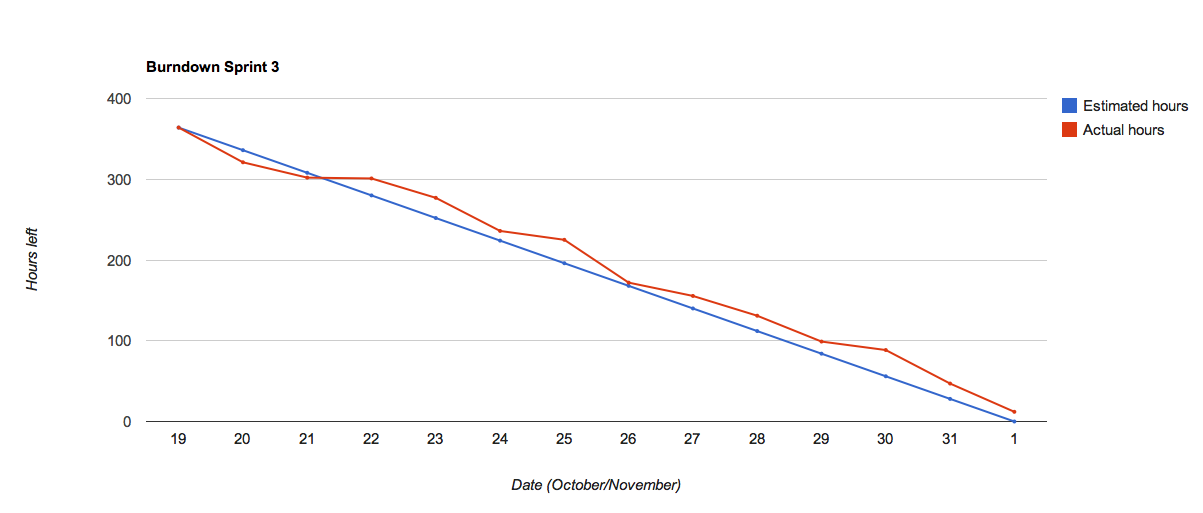
\includegraphics[width=\textwidth]{./sprints/img/burndown_chart_s4}
	\caption{Burndown chart\label{fig:sp4:burndown}}
\end{figure}

The final testing and patching of the utility was done at the customers site. Two of the team members was assigned to this task. To be allowed to see Thales source code, the team members had to sign a non disclosure agreement and be under surveillance of the customer. In addition the customer had a demanding project on their own, so they could not spear many hours for the testing. As it took long time to get the security clearance needed, the testing was blocked until the last week of the sprint. This is listed as a barrier.

\subsection{Positive Experiences}
%--------------------------
\begin{itemize}
\item We all completed a great amount of work.
\item Finished all the items in the sprint backlog.
\item Each team member assigned themselves work items from the backlog, and took responsibility for completing them.
\item Customer is pleased with our work.   
\end{itemize}

\subsection{Negative Experiences}
%--------------------------
\begin{itemize}
\item Meetings were ineffective
\item Slow start this sprint
\item Stumbled into blocked tasks because of dependencies.
\item Too few attendants at the stand-up meetings.
\item Team members took responsibility for more than one task in the backlog at a time. 
\end{itemize}

\subsection{Barriers}
%--------------------------
\subsubsection{External Factors}
The customer asked if we could do a presentation of the utility for the developers at Thales, when it was finished. This would be beneficial for the final presentation and the customer would be pleased, so we accepted. To make the presentation and rehearse for it, two team members had to be excluded from the sprint work for several hours. External factors like this are not always possible to foresee, and it affected the project.

\subsubsection{Thales Security}
It was completely necessary to have Thales source code for the last test- and bug fixing-phase. As a result of the strict rules at Thales, we had to wait with critical implementation and fixing until the middle of the sprint. We managed to have the utility work on their code in the end.
